Бор - корневое дерево, на рёбрах которого написаны символы рассматриваемого алфавита. Если из вершины исходит несколько рёбер, то на них написаны попарно различные символы.

Бор для набора образцов ${he,she,his,hers}$:
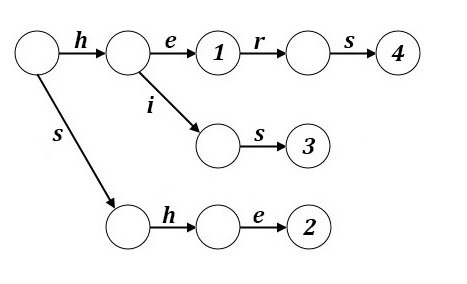
\includegraphics[width=6cm]{images/Бор.jpg}

Пусть нам дан набор слов $s_1, ..., s_n$. Построить бор для такого набора, значит, задать дерево, из корня которого по некоторому пути можно прочитать каждое из этих слов. 

Реализация: 

Построим бор по набору слов $s_1, \dots, s_n$. Для удобства заведём структуру, которая хранит вершину бора.

\begin{lstlisting}
struct node {
  map<char, int> to;
  bool term; // is node terminal? is there the final letter?
};
\end{lstlisting}

Далее заведём сам бор:

\begin{lstlisting}
vector<node> trie;
\end{lstlisting}

Реализация процедуры добаления слова в бор:

\begin{lstlisting}
void add(const string &s) {
  int v = 0;
  for (int i = 0; i < s.size(); ++i) {
    if (!trie[v].to.count(s[i])) {
      trie.push_back(node());
      trie[v].to[s[i]] = int(trie.size()) - 1;
    }
    v = trie[v].to[s[i]];
  }
  trie[v].term = true;
}
\end{lstlisting}

\Note Вместо $map$ подойдут и другие структуры. Например, можно использовать массив длины $|\Sigma|$, где несуществующие значения заполнены $-1$. Подойдёт так же и хеш-таблица.

Сравним их по памяти. Массив: $|\Sigma|$, $map$ и хеш-таблица: $k$ (число исходящих из вершины рёбер).

Сколько нужно ждать выполнения запроса? Массив: $O(1)$. $map$: $O(log k)$. Хеш-таблица: $O(1)$ в среднем.